\chapter[BLOCk input form]{BLOCk input form}
\label{appxb}

\section{\texttt{NSIDE} list of control points}

The side nodes for a patch of NURBS is a list of control point numbers.
The data is given by
\setlength{\baselineskip}{12pt}
\begin{verbatim}
       NSIDes
         side  s1 lside1 k1 (cp1(i),i=1,lside1)
         side  s2 lside2 k2 (cp2(i),i=1,lside2)
           .....
           ! terminate with blank record
\end{verbatim}
\setlength{\baselineskip}{14pt}
where \texttt{s1} is the side number, \texttt{lside1} is the number of
control point numbers in the side vector, \texttt{k1} is the number of
the knot vector associated with the side; and
\texttt{cp1(i)} is the list of \texttt{lside1} control point numbers
defining the
side.  The number of control points and the number of associated knot values
is related by
\begin{verbatim}
       lknot(k1) = lside(s1) + order(k1) + 1
\end{verbatim}
Thus, a linear side (order = 1) with two (2) control points has a knot vector
with four (4) values.  The open knot vector has repeated first and last values
and thus is the form
\begin{verbatim}
       0.0  0.0  1.0  1.0
\end{verbatim}
or similar.

\section{\texttt{NBLOCK} specification}

\begin{figure}[b!]
\begin{center}

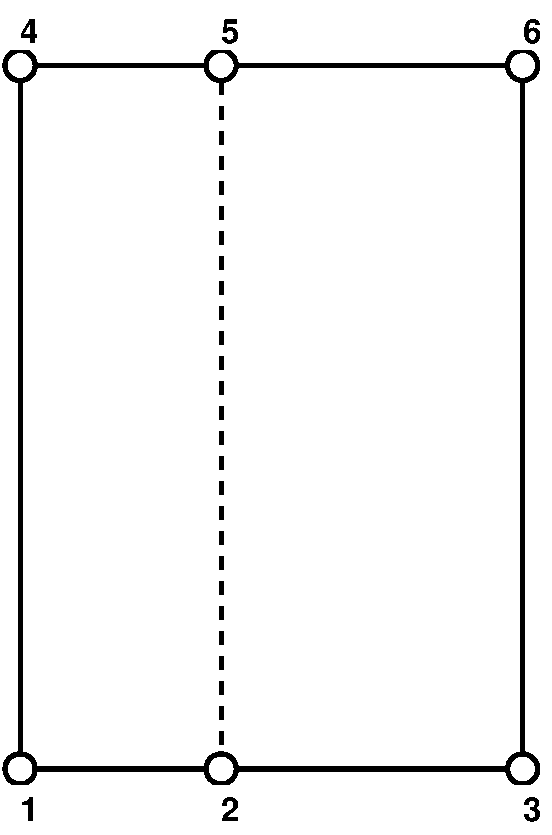
\includegraphics[height=2in]{figs/nblock2d}

\caption{Two dimensional NURBS block data \label{afig2b} }
\end{center}
\end{figure}

\subsection{One dimensional block}

For a one dimensional block the command is given as
\begin{verbatim}
       NBLOck
         block 1 ma side
\end{verbatim}
where \texttt{ma} is the block material set number
and \texttt{side} the side number giving the list of control points.

\subsection{Two dimensional block}

A two dimensional block is described by two knot vectors.  The first knot
vector describes the two sides of the block and also any intermediate list
of sides in the interior of the block directed in the same direction.  The
second knot vector describes the second direction in the block.  The associated
control points for the second knot vector must be the first control point
from all the sides comprising the first direction and given in the order
corresponding to increasing knot values in the second direction.  The
input data for the block is given as
\setlength{\baselineskip}{12pt}
\begin{verbatim}
       NBLOck
         block 2 ma side2
\end{verbatim}
\setlength{\baselineskip}{14pt}
where \texttt{ma} the material set number and
\texttt{side2} the side number for the second block direction.
For example, the block shown in Fig. \ref{afig2b} can let block direction 1
be associated with side with control points 1 and 4 and block direction 2 with
control points 1, 2, and 3.

\begin{quote}
\noindent
\textbf{Example: 2-d NURB BLOCK}

The data for the two dimensional tensor product block shown in
Figure \ref{afig2b} is specified as follows:

\begin{minipage}{\textwidth}
\setlength{\baselineskip}{12pt}
\begin{verbatim}
       NURBs
         1  0   0.0   0.0  1.0
         2  0  40.0   0.0  1.0
         3  0 100.0   0.0  1.0
         4  0   0.0 140.0  1.0
         5  0  40.0 140.0  1.0
         6  0 100.0 140.0  1.0

       KNOTs
         open 1  4  0.0 0.0 1.0 1.0
         open 2  5  0.0 0.0 0.5 1.0 1.0

       NSIDEs
         side 1  2  1  1  4
         side 2  2  1  2  5
         side 3  2  1  3  6
         side 4  3  2  1  2  3

       NBLOCK
         block  2  1  4

\end{verbatim}
\setlength{\baselineskip}{14pt}
\end{minipage}

Note that the specification of the dotted line at the knot value 0.5 is
not necessary to give an exact geometry for this simple rectangle.  However,
it permits for a non-uniform subdivision in the horizontal direction later.
\end{quote}

\subsection{Three dimensional block}

\setlength{\baselineskip}{16pt}
The specification of a three dimensional NURBS block is given by defining the
list of all the sides lists for one of the block directions.
In Fig. \ref{afig3b} the sides in the 3 knot-direction are used to define
a rectangular block.  The NURBS block command for a three dimensional block
is given as

\setlength{\baselineskip}{12pt}
\begin{verbatim}
       NBLOCK
         block 3 ma k1 k2
         (side(i),i = 1,list3d)
\end{verbatim}
\setlength{\baselineskip}{14pt}
where \texttt{ma} is the material set number; \texttt{k1, k2} are the knot
numbers defining the generator plane of the block; and \texttt{side(i)} is the
list of sides perpendicular to the generator plane.

\begin{quote}
\noindent{\textbf{Example: Three dimensional rectangular block}}

The data for the rectangular block shown in Fig. \ref{afig3b} is given by
the control point locations for nodes 1 to 12 and the following knot vectors;
side lists; and block command:

\begin{minipage}{\textwidth}
\setlength{\baselineskip}{12pt}
\begin{verbatim}
       KNOTS
         open 1  6  0.0 0.0 0.0 1.0 1.0 1.0
         open 2  4  0.0 0.0 1.0 1.0
         open 3  4  0.0 0.0 1.0 1.0

       NSIDES
         side 1  2  3   1  2
         side 2  2  3   3  4
         side 3  2  3   5  6
         side 4  2  3   7  8
         side 5  2  3   9 10
         side 6  2  3  11 12

       NBLOCK
         block 3 1  1  2
           1 2 3 4 5 6

\end{verbatim}
\setlength{\baselineskip}{14pt}
\end{minipage}

\begin{figure}[b!]
\begin{center}

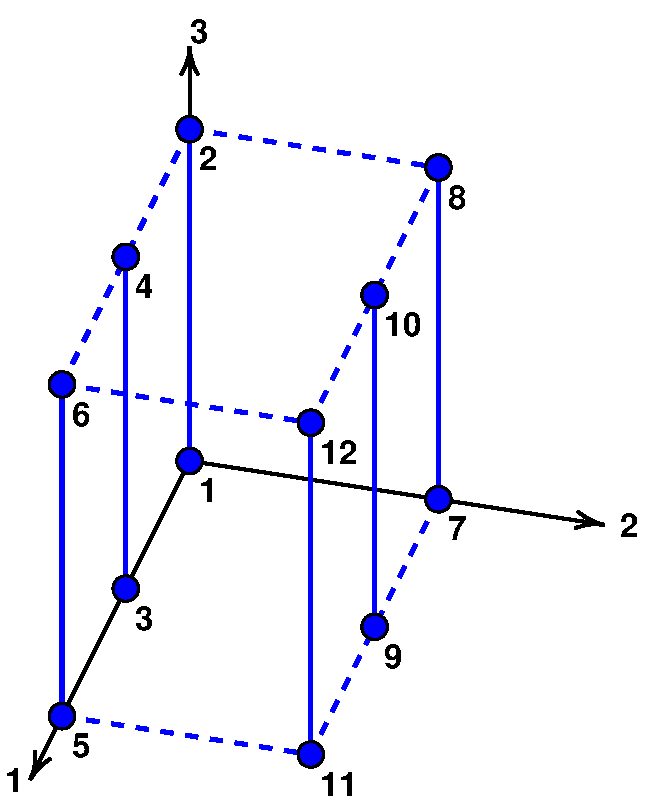
\includegraphics[height=2.5in]{figs/nblock3d}

\caption{Three dimensional NURBS block data \label{afig3b} }
\end{center}
\end{figure}

The direction 1 of the block is
a quadratic NURBS while directions 2 and 3 are linear NURBS.
Since the 1-direction is quadratic, the first 3 side lists will be used to
define this direction while the second set of three will create the linear
behavior for the 2-direction.
\end{quote}
